\providecommand{\main}{..}
\documentclass[\main/TL_liquid.tex]{subfiles}
\graphicspath{{\main/images/}}
\setcounter{section}{1}
\begin{document}
\section{Jacobiの三重積}

\begin{frame}{マヤ図形}
    整数に$\bullet,\circ$のいずれかを対応づけるような写像
    \begin{align}
        M: \mathbb{Z} \to \{\bullet,\circ\}
    \end{align}
    であって、$k \gg 0$で
    \begin{align}
        M(-k) = \bullet, \quad
        M(k) = \circ
    \end{align}
    を満たすものをマヤ図形と呼ぶ。
    これを以下のように図示する。
    \begin{figure}[H]
        \centering
        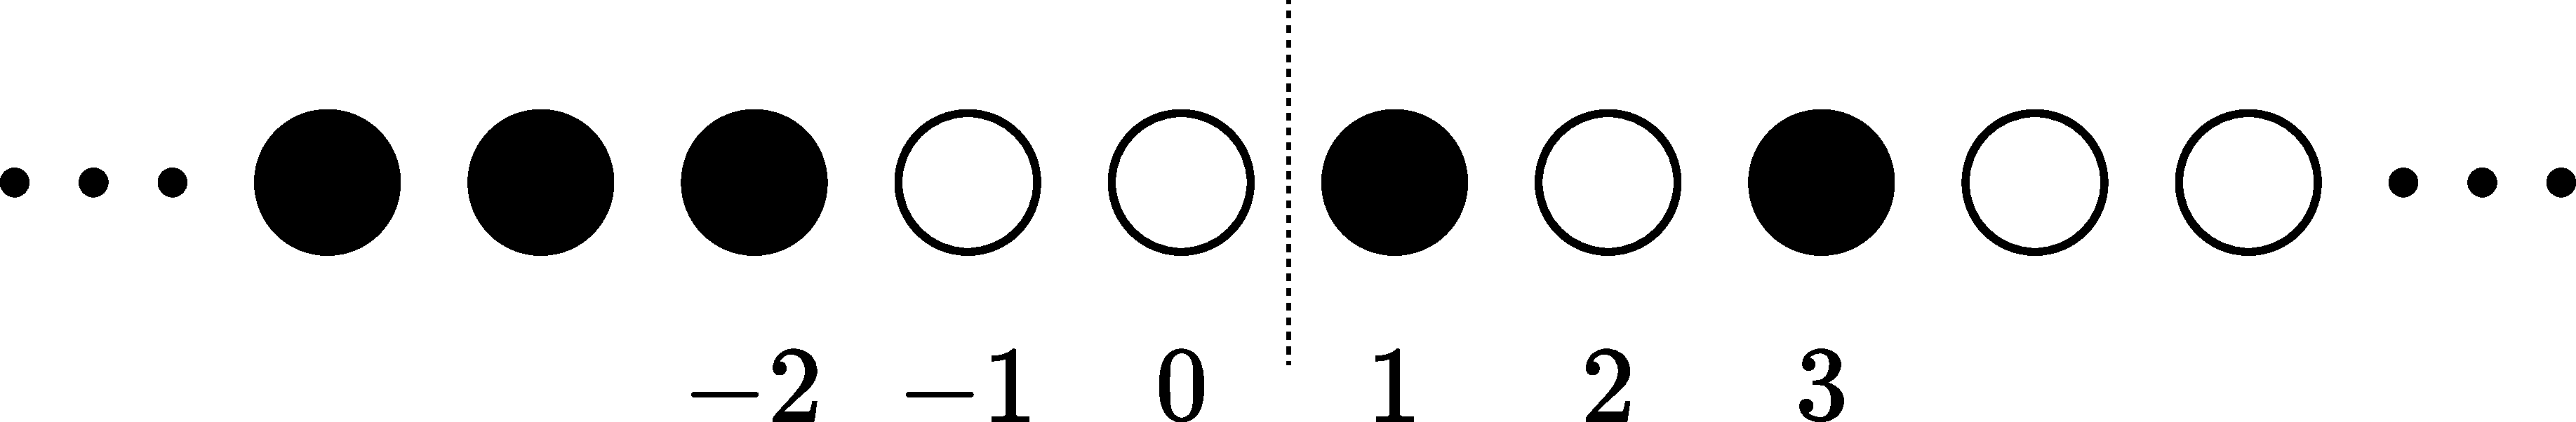
\includegraphics[scale = 0.1]{Maya.pdf}
    \end{figure}
    $k>0$の領域にある$\bullet$を\alert{電子}と呼び、$k\le0$の領域にある$\circ$を\alert{ホール}と呼ぶ。
\end{frame}

\begin{frame}{電荷とエネルギー}
    マヤ図形$M$の電荷を
    \begin{align}
        Q(M) = (\text{電子の総数}) - (\text{ホールの総数})
    \end{align}
    と定義する。

    電子が$k > 0$にいるとき、その電子のエネルギーを$k$と定義する。
    またホールが$k \le 0$にいるとき、そのホールのエネルギーを$-k$と定義する。
    マヤ図形のエネルギーを
    \begin{align}
        E(M) = (\text{電子のエネルギーの総和}) + (\text{ホールのエネルギーの総和})
    \end{align}
    によって定義する。
\end{frame}

% \begin{frame}{生成消滅演算子}
%     \begin{align}
%         E = \frac{1}{2}Q(Q+1) + N
%         \equiv E_0 + N
%     \end{align}
% \end{frame}

\begin{frame}{Young図形とマヤ図形の対応関係}
    \begin{figure}[H]
        \centering
        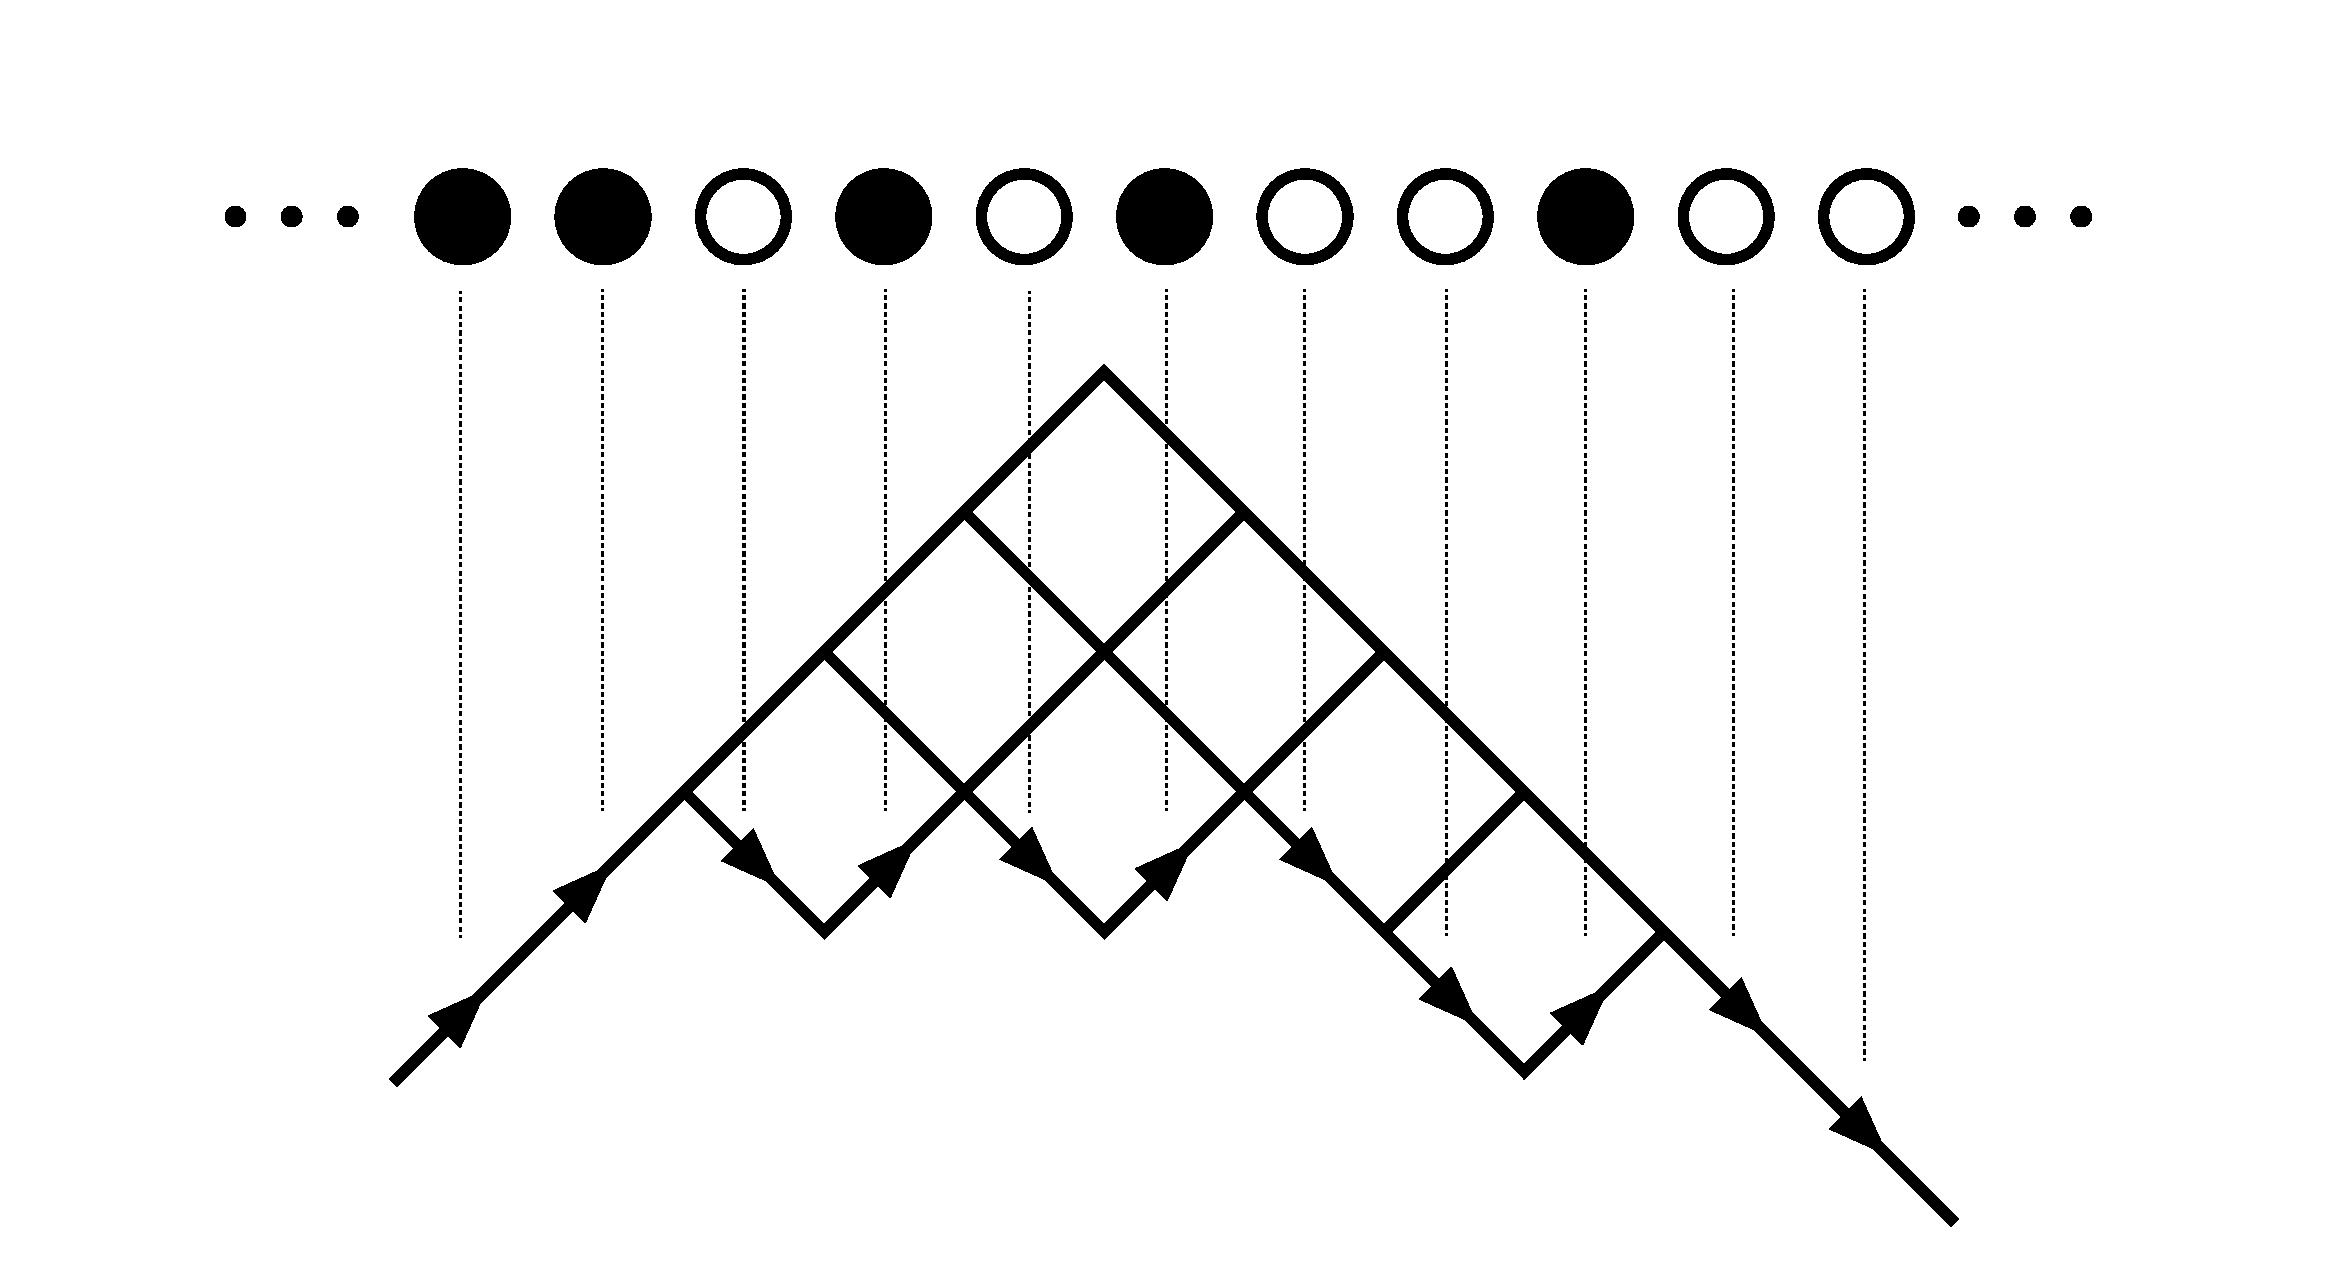
\includegraphics[scale = 0.2]{relation.pdf}
    \end{figure}
    上図のように、マヤ図形にYoung図形を対応付けることができる。またYoung図形から原点の自由度を除いてマヤ図形を決定することができる。

    このようにして、マヤ図形の集合$\mathcal{M}$と、
    整数とヤング図形の集合の直積集合$\mathbb{Z} \times Y$との間の全単射が得られる。
\end{frame}

\begin{frame}{Young図形とマヤ図形の対応関係}
    基底状態を以下のように設定する。
    \begin{figure}[H]
        \centering
        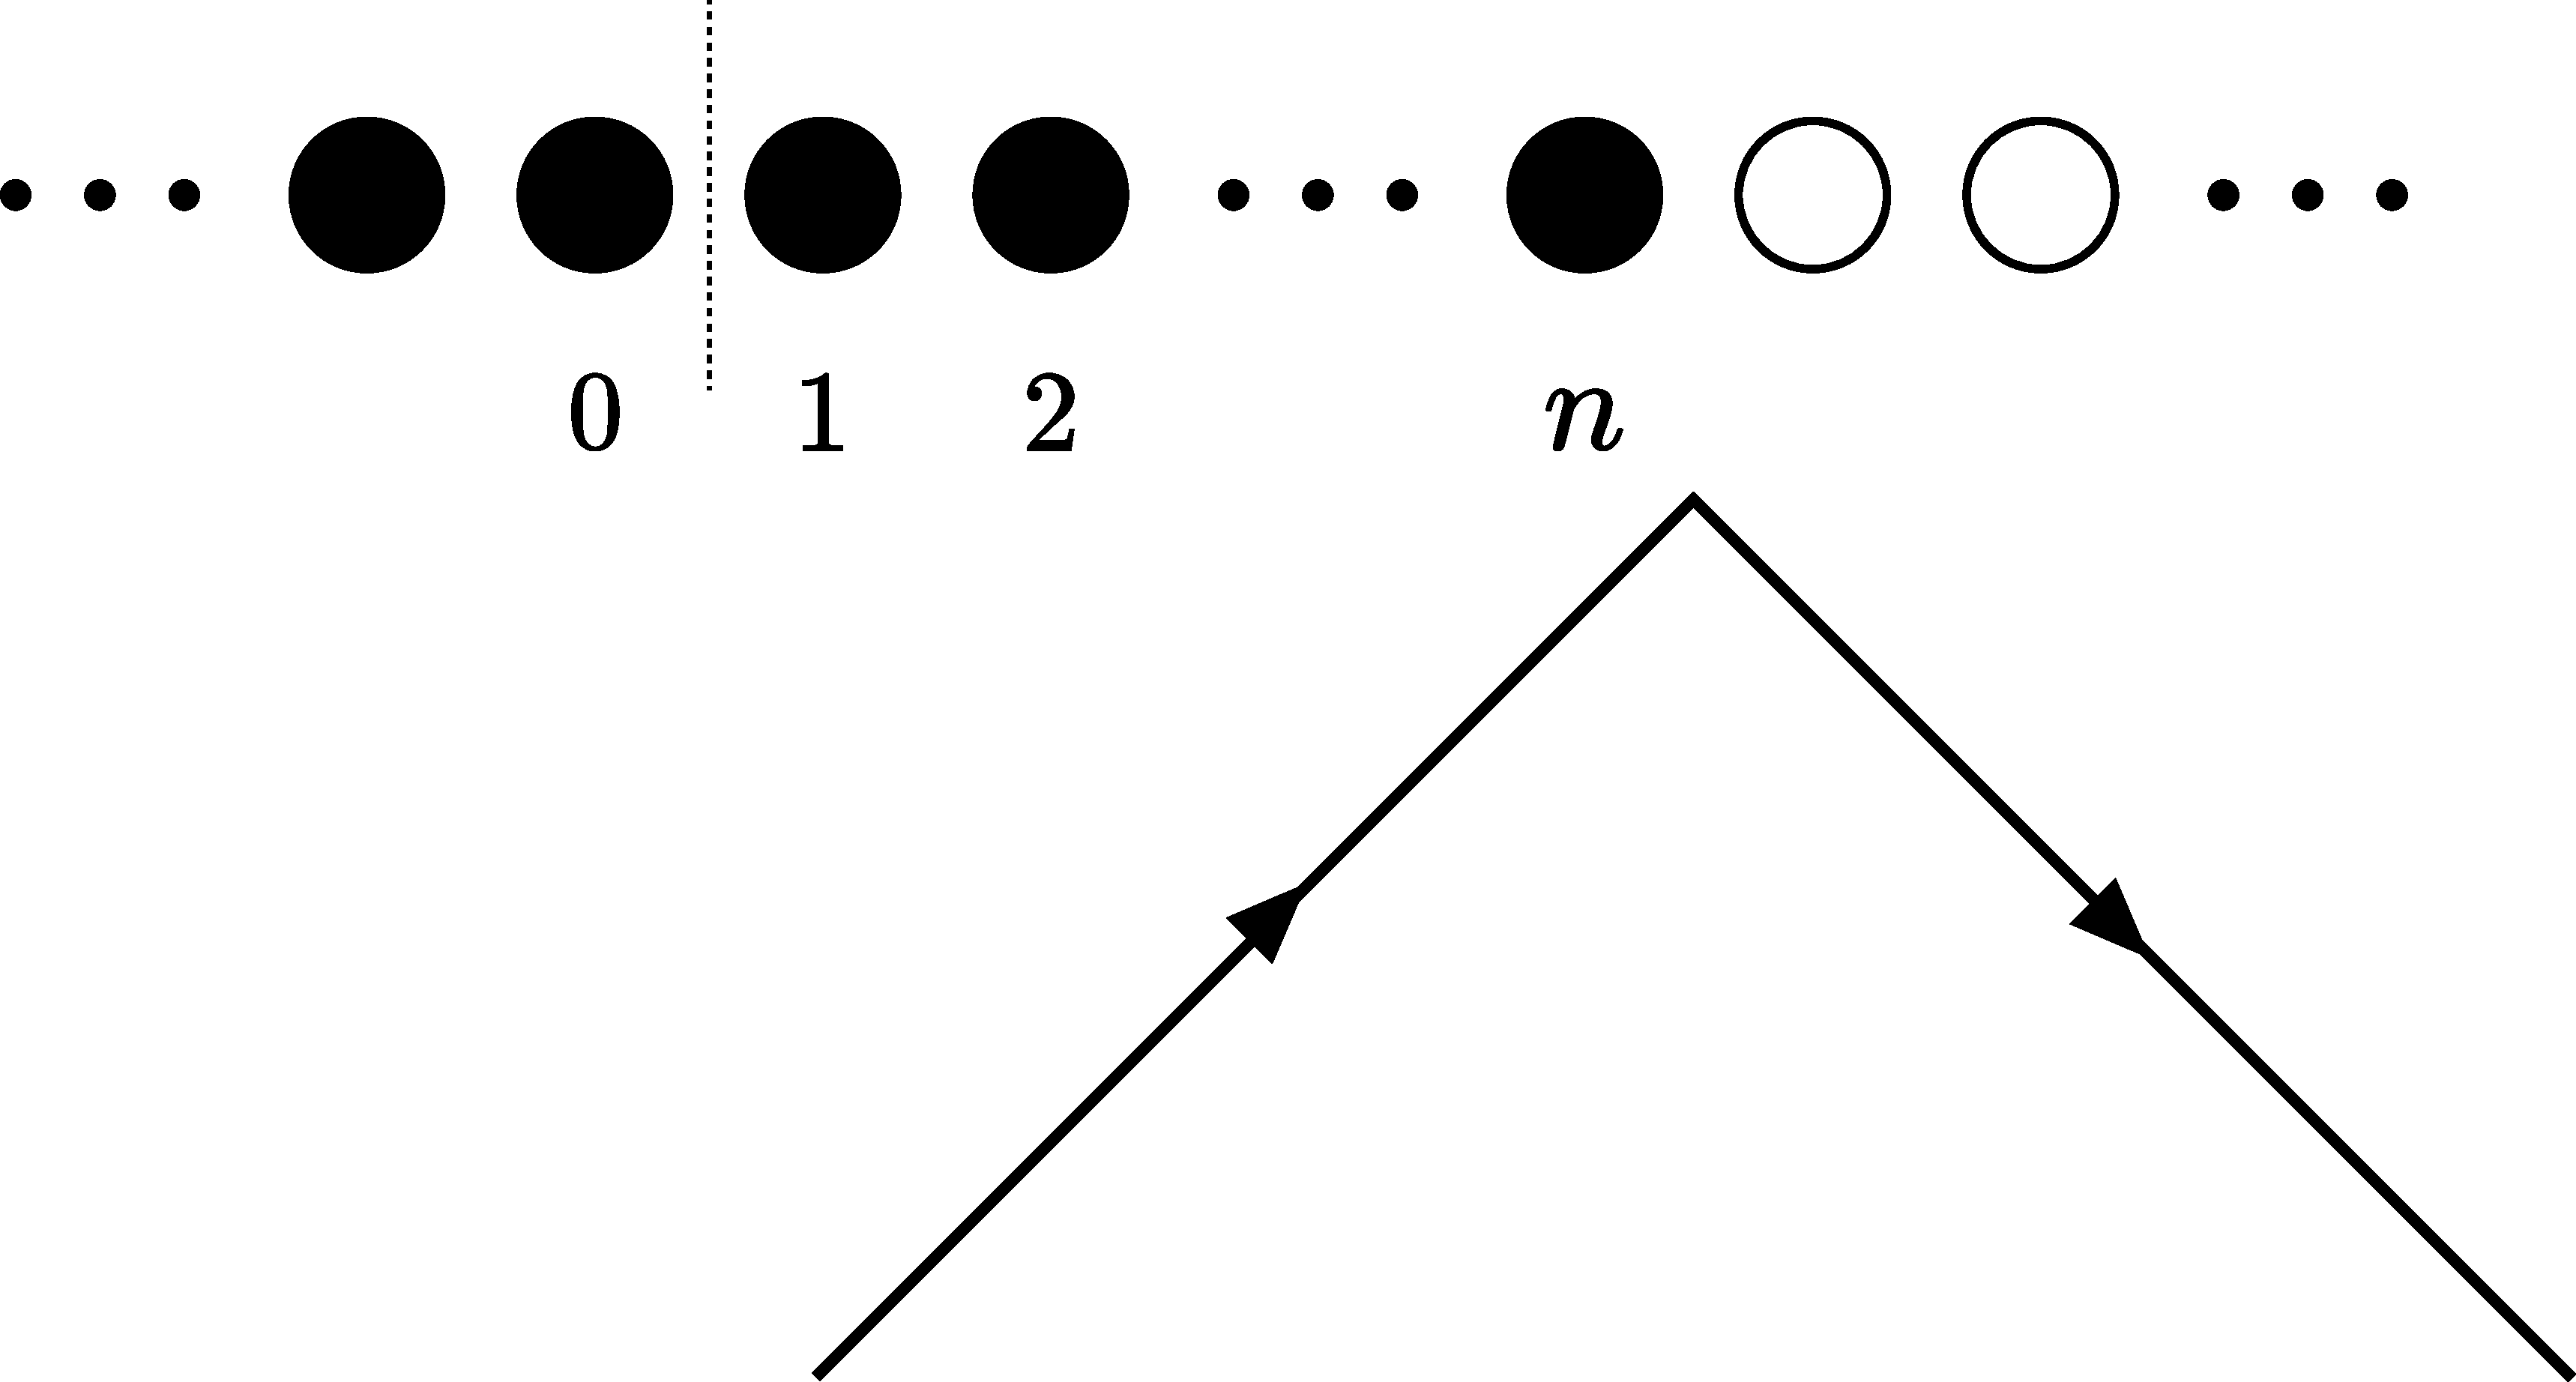
\includegraphics[scale = 0.12]{gnd.pdf}
    \end{figure}
    基底状態の電荷を$n$とすると、エネルギーは$n(n+1)/2$である。
\end{frame}

\begin{frame}{Young図形とマヤ図形の対応関係}
    基底状態に以下で定義する操作$a_{k+1}^\dagger a_k$を繰り返すことで、任意のマヤ図形およびYoung図形を構成できる。
    \begin{figure}[H]
        \centering
        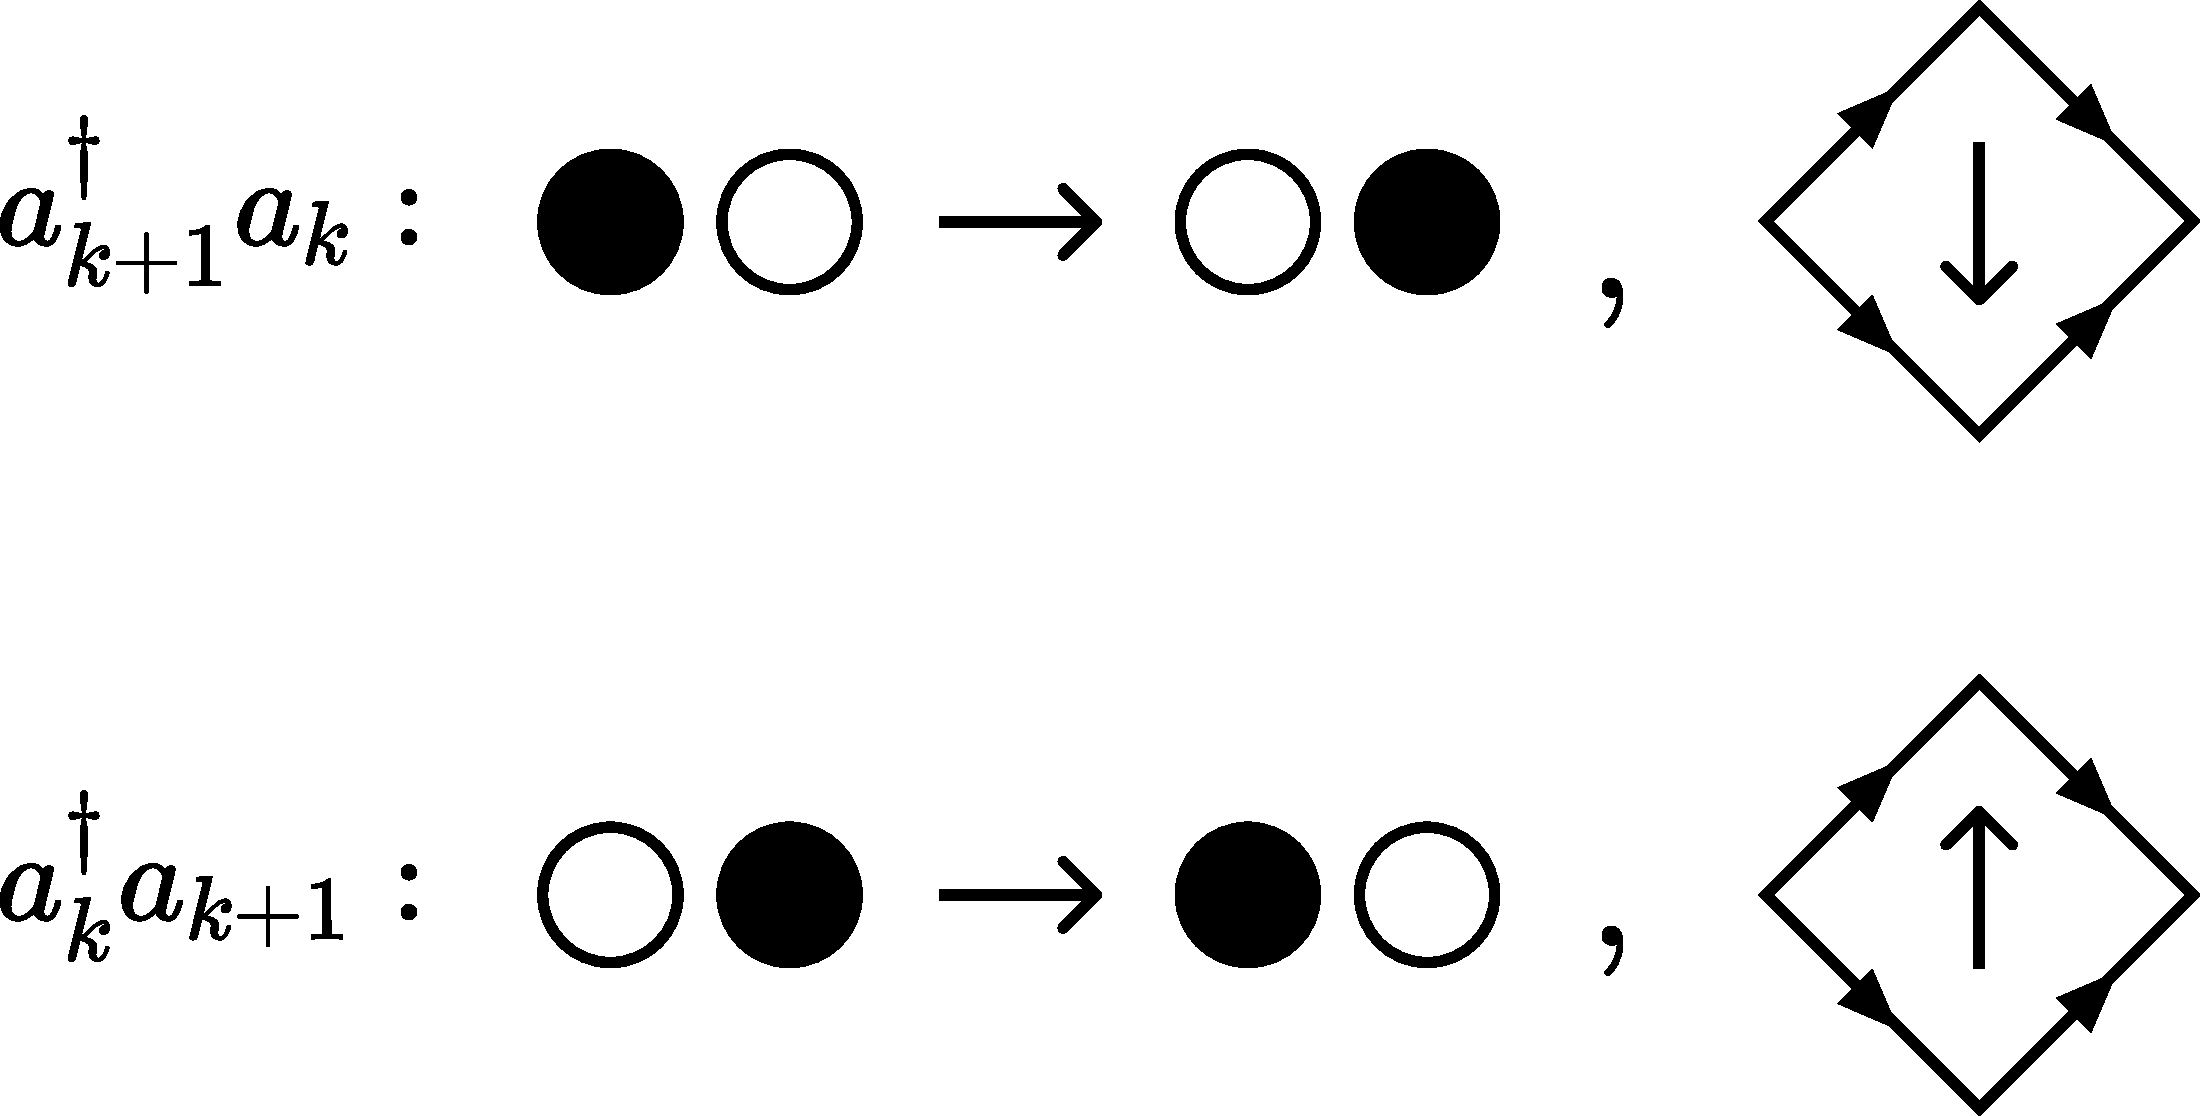
\includegraphics[scale = 0.15]{tranfer.pdf}
    \end{figure}
    基底状態に$a_{k+1}^\dagger a_k$を$N$回掛けた場合にあり得るマヤ図形の数は、大きさ$N$のYoung図形の数$p(N)$に一致する。
\end{frame}

\begin{frame}{Jacobiの三重積}
    マヤ図形に対する母関数を考える。
    Young図形とマヤ図形の対応関係から、マヤ図形を$(N,Q)$によってラベル付けすると、
    \begin{align}
        \sum_{M \in \mathcal{M}} q^{E(M)}z^{Q(M)}
        =
        \sum_{n\in\mathbb{Z}} \sum_{N=0}^\infty p(N)q^{E_0+N} z^{n}
    \end{align}
    となる。
    ただし$E_0 = n(n+1)/2$である。
    一方、$k\in \mathbb{Z}$に$\bullet$があるか$\circ$があるかによってマヤ図形をラベル付けすると、
    \begin{align}
        \sum_{M \in \mathcal{M}} q^{E(M)}z^{Q(M)}
        =
        \prod_{k = 0}^\infty (1+q^{k} z^{-1}) \prod_{k=1}^\infty (1+q^k z)
    \end{align}
    となる。
\end{frame}

\begin{frame}{Jacobiの三重積}
    \begin{align}
        \sum_{n\in\mathbb{Z}} \sum_{N=0}^\infty p(N)q^{E_0+N} z^{n}
        = \prod_{k=1}^\infty \frac{1}{1-q^k} \sum_{n \in \mathbb{Z}} q^{n(n+1)/2}z^n
    \end{align}
    \begin{align}
        \prod_{k = 0}^\infty (1+q^k z^{-1}) \prod_{k=1}^\infty (1+q^k z)
        = \prod_{k=1}^\infty (1+q^{k-1}z^{-1})(1+q^kz)
    \end{align}
    2つを等号で結ぶことで、
    \begin{align}
        \sum_{n\in \mathbb{Z}} q^{n(n+1)/2}z^n
        = \prod_{k=1}^{\infty}
            (1-q^{k})(1+q^{k}z)(1+q^{k-1}z^{-1})
        \label{Jacobi triple product}
    \end{align}
    となって、Jacobiの三重積が証明された。
\end{frame}

% \begin{frame}{Jacobiの三重積の背景}
%     Jacobiの三重積は無限次元のLie環に関係しているらしい。
% \end{frame}
\end{document}